\documentclass{standalone}

\usepackage{ tikz }
\usetikzlibrary{automata, positioning, arrows}

\newcommand{\trs}[2]{#1 \,|\, #2}

\begin{document}
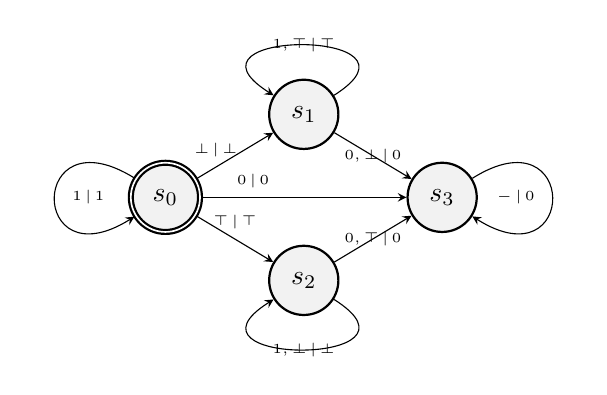
\begin{tikzpicture}[->, >=stealth, node distance=3cm, every state/.style={thick, fill=gray!10}, initial text=$ $, every edge/.append style={font=\tiny}, yscale=-1, x=100pt, y=30pt]
    \node[state, accepting] (s0) at (0,0) {\(s_0\)};
    \node[state] (s1) at (0.5,-1) {\(s_1\)};
    \node[state] (s2) at (0.5,1) {\(s_2\)};
    \node[state] (s3) at (1,0) {\(s_3\)};

    \draw (s0) edge[above] node[near start]{\(\trs{\bot}{\bot}\)} (s1);
    \draw (s0) edge[above] node[near start]{\(\trs{0}{0}\)} (s3);
    \draw (s0) edge[above] node{\(\trs{\top}{\top}\)} (s2);
    \draw (s0) edge[out=225, in=135, loop, distance=2cm] node[right=0.1cm]{
        \(\trs{1}{1}\)
    } (s0);

    \draw (s1) edge node{\(\trs{0, \bot}{0}\)} (s3);
    \draw (s1) edge[out=315, in=225, loop, distance=2cm] node{
        \(\trs{1, \top}{\top}\)
    } (s1);

    \draw (s2) edge node{\(\trs{0, \top}{0}\)} (s3);
    \draw (s2) edge[out=45, in=135, loop, distance=2cm] node{
        \(\trs{1, \bot}{\bot}\)
    } (s2);

    \draw (s3) edge[out=315, in=45, loop, distance=2cm] node[left=0.1cm]{
        \(\trs{-}{0}\)
    } (s3);
\end{tikzpicture}
\end{document}